\documentclass[11pt]{amsart}
\usepackage{amssymb,amsthm,mathtools}
\usepackage{graphicx}
\usepackage[colorlinks=true,linkcolor=blue,citecolor=blue,urlcolor=blue]{hyperref}

\numberwithin{equation}{section}

\newtheorem{theorem}{Theorem}[section]
\newtheorem{proposition}[theorem]{Proposition}
\newtheorem{lemma}[theorem]{Lemma}
\newtheorem{corollary}[theorem]{Corollary}
\theoremstyle{definition}
\newtheorem{example}[theorem]{Example}
\theoremstyle{remark}
\newtheorem{remark}[theorem]{Remark}

\newcommand{\R}{\mathbb{R}}
\newcommand{\Sph}{\mathbb{S}}
\newcommand{\Tr}{\operatorname{Tr}}
\newcommand{\dd}{\,\mathrm{d}}
\newcommand{\FC}[1]{\mathcal{F}_{#1}}
\newcommand{\Ct}{\widetilde{C}_t}
\newcommand{\taut}{\widetilde{\tau}_t}
\newcommand{\ip}[2]{\langle #1,#2\rangle}
\newcommand{\hatf}[1]{\widehat{#1}}
\newcommand{\tp}{\top}

\begin{document}

\title[Koopman invariance of Gaussian RKHSs]{Koopman invariance of Gaussian RKHSs for linear stochastic
differential equations: a necessary and sufficient condition}

% Author data to be completed by the submitting author:
% \author{First Last}
% \address{Institution, Address}
% \email{name@example.org}

\subjclass[2020]{Primary 46E22, 47D07; Secondary 60H10, 47B33, 42B10}
\keywords{Koopman operator, reproducing kernel Hilbert space, Gaussian kernel, Ornstein--Uhlenbeck process,
Lyapunov inequality, kernel extended dynamic mode decomposition}

\begin{abstract}
Philipp, Schaller, Worthmann, Peitz and N\"uske showed that the reproducing kernel Hilbert space $H_C$ of the
Gaussian kernel $\exp(-\|C^{-1}(x-y)\|^2)$ is invariant under the Koopman semigroup of the linear stochastic
differential equation $\mathrm dX_t=AX_t\,\mathrm dt+B\,\mathrm dW_t$, with $A$ Hurwitz and $(A,B)$ controllable,
whenever $\frac12(AC^2+C^2A^\tp)\le BB^\tp$. They asked whether this condition is also necessary. We show that it is not,
and we identify the exact condition: $H_C$ is invariant under every Koopman operator $K^t$, $t\ge0$, if and only if
$\frac12(AC^2+C^2A^\tp)\le 2BB^\tp$. For a single time $t$ we prove that $K^t$ maps $H_C$ isomorphically onto the
Gaussian RKHS with matrix $\bigl(e^{-At}(C^2+4\Sigma(t))e^{-A^\tp t}\bigr)^{1/2}$, where $\Sigma(t)$ is the conditional
covariance of $X_t$ given $X_0$. Consequently $K^tH_C\subset H_C$ holds if and only if
$e^{At}C^2e^{A^\tp t}\le C^2+4\Sigma(t)$, and then $\|K^t\|=e^{-t\Tr A/2}$. For Hurwitz $A$ the criterion says
that the ellipsoid of $C^2+4\Sigma$, where $\Sigma$ is the stationary covariance, is forward invariant under
$\dot x=Ax$. The proofs rest on a Fourier description of Gaussian RKHSs, in which $K^t$ becomes a weighted
composition operator.
\end{abstract}

\maketitle

%======================================================================
\section{Introduction}\label{sec:intro}
%======================================================================

The Koopman operator, introduced in \cite{Koopman} for deterministic systems, acts on observables $f$ of a
stochastic dynamical system by $(K^tf)(x)=\mathbb E[f(X_t)\,|\,X_0=x]$. It is linear even when the dynamics are not,
and it can be approximated
from data, for instance by extended dynamic mode decomposition (EDMD) \cite{WilliamsEDMD} and its kernel-based
variants \cite{WilliamsKernel,Klus}; see \cite{Mauroy} for an overview. As pointed out in \cite{PSWPN}, the derivation
of error bounds for kernel-based approximations of Koopman operators \cite{Kostic,PhilippACHA,Koehne} benefits greatly
from the reproducing kernel Hilbert space (RKHS) of the kernel being invariant under the Koopman operator. This raises
the question of which kernels and which systems are compatible in this sense.

Philipp, Schaller, Worthmann, Peitz and N\"uske \cite{PSWPN} studied this question for the linear stochastic
differential equation
\begin{equation}\label{eq:sde}
\mathrm dX_t=AX_t\,\mathrm dt+B\,\mathrm dW_t ,
\end{equation}
where $A\in\R^{d\times d}$, $B\in\R^{d\times m}$ and $W$ is an $m$-dimensional Brownian motion, together with the
Gaussian kernel
\[
k^C(x,y)=\exp\bigl(-(x-y)^\tp C^{-2}(x-y)\bigr)=\exp\bigl(-\|C^{-1}(x-y)\|^2\bigr),\qquad x,y\in\R^d ,
\]
with $C\in\R^{d\times d}$ symmetric positive definite. Let $H_C$ be the RKHS of $k^C$ on $\R^d$, with norm
$\|\cdot\|_C$, and let
\begin{equation}\label{eq:Sigmat}
\Sigma(t):=\int_0^te^{As}BB^\tp e^{A^\tp s}\dd s\qquad(t\ge0)
\end{equation}
be the covariance of $X_t$ given $X_0$. Under the standing assumptions of \cite{PSWPN}, namely $m\le d$, $(A,B)$
controllable and $A$ Hurwitz, they proved \cite[Theorem~2.1]{PSWPN} that the Lyapunov-type inequality
\begin{equation}\label{eq:23}
\tfrac12\bigl(AC^2+C^2A^\tp\bigr)\le BB^\tp
\end{equation}
(in the Loewner order; this is \cite[(2.3)]{PSWPN}) implies $K^tH_C\subset H_C$ for all $t\ge0$, with
$\|K^tf\|_C\le e^{-t\Tr A/2}\|f\|_C$. Whether \eqref{eq:23} is also necessary was left open
\cite[Remark~2.2(c) and Remark~4.2]{PSWPN}.

\subsection*{Main result}
The answer is negative. The following theorem characterizes invariance completely, both at a fixed time and for
the whole semigroup. It needs none of the standing assumptions of \cite{PSWPN}.

\begin{theorem}\label{thm:main}
Let $A\in\R^{d\times d}$ and $B\in\R^{d\times m}$ be arbitrary, and let $C\in\R^{d\times d}$ be symmetric positive
definite.
\begin{enumerate}
\item[(a)] For every $t\ge0$,
\begin{equation}\label{eq:critA}
K^tH_C\subset H_C\iff e^{At}C^2e^{A^\tp t}\le C^2+4\Sigma(t),
\end{equation}
and in this case $\|K^t\|_{H_C\to H_C}=e^{-t\Tr A/2}$.
\item[(b)] $K^tH_C\subset H_C$ holds for every $t\ge0$ if and only if
\begin{equation}\label{eq:23sharp}
\tfrac12\bigl(AC^2+C^2A^\tp\bigr)\le 2BB^\tp .
\end{equation}
If \eqref{eq:23sharp} fails, there is $\varepsilon>0$ such that $K^tH_C\not\subset H_C$ for every
$t\in(0,\varepsilon)$.
\end{enumerate}
\end{theorem}

Here $K^tf$ is defined pointwise by $(K^tf)(x)=\mathbb E[f(X_t)\,|\,X_0=x]$, which makes sense for the bounded
continuous functions in $H_C$. Under the standing assumptions of \cite{PSWPN} this agrees with their definition on
$L^2(\mu)$, $\mu$ the stationary distribution (Remark~\ref{rem:L2mu}).

\begin{corollary}[Answer to the question of \cite{PSWPN}]\label{cor:answer}
Condition \eqref{eq:23} implies \eqref{eq:23sharp}, but not conversely. For instance,
\[
A=\begin{pmatrix}-1&5\\0&-1\end{pmatrix},\qquad B=C=I_2
\]
satisfy all standing assumptions of \cite{PSWPN} and \eqref{eq:23sharp}, but not \eqref{eq:23}. Hence \eqref{eq:23} is
sufficient but not necessary for $K^tH_C\subset H_C$, $t\ge0$. Condition \eqref{eq:23sharp} is exactly
condition \eqref{eq:23} for the matrix $C/\sqrt2$ in place of $C$.
\end{corollary}

\subsection*{Idea of the proof}
Gaussian RKHSs are weighted $L^2$-spaces in Fourier variables: $f\in H_C$ if and only if
$\int|\hatf f(\xi)|^2e^{\frac14\xi^\tp C^2\xi}\dd\xi<\infty$ (Lemma~\ref{lem:fourier}). In Fourier variables, $K^t$
acts by composition with the linear map $e^{-A^\tp t}$, followed by multiplication with the Gaussian
$\exp(-\frac12\xi^\tp e^{-At}\Sigma(t)e^{-A^\tp t}\xi)$ and the constant $e^{-t\Tr A}$ (Lemma~\ref{lem:Kt}). Invariance therefore amounts to comparing two Gaussian weights, i.e.\ two quadratic forms.
This comparison gives \eqref{eq:critA}, and differentiating \eqref{eq:critA} at $t=0$ gives \eqref{eq:23sharp}.

\subsection*{Where the factor two comes from}
The proof in \cite{PSWPN} tracks kernel sections. The function $k^C_z=k^C(z,\cdot)$ is a Gaussian bump with
``covariance'' $\frac12C^2$, and averaging over the transition law adds $\Sigma(t)$ to it. This gives
$K^tk^C_z=\tau_t\,k^{C_t}_{e^{-At}z}$ with $C_t:=\bigl(e^{-At}(C^2+2\Sigma(t))e^{-A^\tp t}\bigr)^{1/2}$ and a constant
$\tau_t>0$ \cite[Proposition~4.1]{PSWPN}. Consequently $K^t$ maps $H_C$ into $H_{C_t}$, and \eqref{eq:23} is
equivalent to $H_{C_t}\subset H_C$ for all $t\ge0$. Membership in $H_C$, however, is decided by $|\hatf f|^2$. In
$|\hatf f|^2$ the Gaussian factor produced by the averaging appears \emph{squared}. As a result, the range of $K^t$
is the space $H_{\Ct}$ with $\Ct^{\,2}=e^{-At}(C^2+4\Sigma(t))e^{-A^\tp t}$ (Theorem~\ref{thm:range}), which is strictly
smaller than $H_{C_t}$ when $t>0$ and $B\ne0$. Invariance is equivalent to $H_{\Ct}\subset H_C$, which replaces $2\Sigma(t)$ by
$4\Sigma(t)$ and $BB^\tp$ by $2BB^\tp$. Finite kernel expansions cannot see the difference
(Remark~\ref{rem:sections}). The functions that $K^t$ maps out of $H_C$ have Fourier transforms that decay as
slowly as membership in $H_C$ permits, within a cone of directions (Lemma~\ref{lem:multiplier}).

\subsection*{Stable drift}
If $A$ is Hurwitz, then $\Sigma:=\lim_{t\to\infty}\Sigma(t)$ exists and $A\Sigma+\Sigma A^\tp=-BB^\tp$. In this case
\eqref{eq:23sharp} is equivalent to $A(C^2+4\Sigma)+(C^2+4\Sigma)A^\tp\le0$, whereas \eqref{eq:23} is equivalent
to $A(C^2+2\Sigma)+(C^2+2\Sigma)A^\tp\le0$. Geometrically, $H_C$ is invariant if and only if the ellipsoid
$\{x:\,x^\tp(C^2+4\Sigma)^{-1}x\le1\}$ is forward invariant under $\dot x=Ax$ (Theorem~\ref{thm:D}). Moreover, for
every $C$, invariance holds for all sufficiently large $t$. Figure~\ref{fig:times} shows the admissible times for
a family of examples.

\subsection*{Beyond Gaussian kernels}
The Fourier approach applies to every translation-invariant kernel with a positive integrable spectral density
(Proposition~\ref{prop:general}). For instance, Sobolev (Mat\'ern) RKHSs are invariant for all $A$ and $B$
(Example~\ref{ex:sobolev}). A Lyapunov-type restriction thus appears because the spectral density of a Gaussian kernel is
itself Gaussian.

\subsection*{Organization}
Section~\ref{sec:fourier} describes Gaussian RKHSs in Fourier variables, and Section~\ref{sec:koopman} does the
same for the Koopman operators. Section~\ref{sec:proofs} proves Theorem~\ref{thm:main} and
Corollary~\ref{cor:answer} and determines the range of $K^t$. Section~\ref{sec:geometry} treats Hurwitz drifts,
Section~\ref{sec:examples} contains examples, and Section~\ref{sec:remarks} collects further remarks, including
other kernels. Appendix~\ref{app:numerics} lists numerical checks of the identities.

\subsection*{Notation}
For symmetric matrices, $P\le Q$ means that $Q-P$ is positive semidefinite, and $P>0$ that $P$ is positive definite.
$|x|$ is the Euclidean norm, $\|M\|$ the spectral norm, $M^{-\tp}:=(M^{-1})^\tp$, $\Sph^{d-1}$ the unit sphere and
$\mathbf 1_E$ the indicator function of a set $E$. For $x\in\R^d$ we write $k^C_x:=k^C(x,\cdot)$.

%======================================================================
\section{Gaussian RKHSs in Fourier variables}\label{sec:fourier}
%======================================================================

For $g\in L^1(\R^d)$ let $\hatf g(\xi):=\int_{\R^d}g(x)e^{-i\xi\cdot x}\dd x$. The map $g\mapsto\hatf g$ extends
to $L^2(\R^d)$ with $\|\hatf g\|_{L^2}^2=(2\pi)^d\|g\|_{L^2}^2$ (Plancherel). For $F\in L^1(\R^d)\cap L^2(\R^d)$ put
$F^\vee(x):=(2\pi)^{-d}\int F(\xi)e^{i\xi\cdot x}\dd\xi$. Then $F^\vee$ is continuous, $F^\vee\in L^2(\R^d)$ and
$\hatf{F^\vee}=F$. If $g\in L^2(\R^d)\cap C(\R^d)$ and $\hatf g\in L^1(\R^d)$, then $g=(\hatf g)^\vee$ everywhere,
since both functions are continuous and agree almost everywhere. A measurable function $F$ is \emph{Hermitian} if
$F(-\xi)=\overline{F(\xi)}$ for a.e.\ $\xi$. If $g$ is real-valued, then $\hatf g$ is Hermitian. If
$F\in L^1\cap L^2$ is Hermitian, then $F^\vee$ is real-valued. For $P>0$ and $\xi\in\R^d$ we use the Gaussian integral
\begin{equation}\label{eq:gauss}
\int_{\R^d}\exp\bigl(-x^\tp Px-i\xi\cdot x\bigr)\dd x=\pi^{d/2}(\det P)^{-1/2}\exp\bigl(-\tfrac14\xi^\tp P^{-1}\xi\bigr),
\end{equation}
which reduces to $\int_\R e^{-px^2-i\xi x}\dd x=\sqrt{\pi/p}\,e^{-\xi^2/(4p)}$ after an orthogonal diagonalization of $P$.

For symmetric positive definite $C$ we define
\begin{equation}\label{eq:wC}
w_C(\xi):=\exp\bigl(\tfrac14\xi^\tp C^2\xi\bigr),\qquad \kappa_C:=\pi^{d/2}\det C,\qquad
\FC{C}:=\Bigl\{F:\R^d\to\mathbb C\ \text{measurable and Hermitian}:\ \int|F|^2w_C\dd\xi<\infty\Bigr\}.
\end{equation}
By \eqref{eq:gauss} with $P=C^{-2}$, followed by a translation,
\begin{equation}\label{eq:kernelFT}
\hatf{k^C_y}(\xi)=\kappa_C\,e^{-i\xi\cdot y}\,w_C(\xi)^{-1},\qquad y,\xi\in\R^d ,
\end{equation}
and by \eqref{eq:gauss} with $\xi=0$ and $P=\frac14C^2$,
\begin{equation}\label{eq:intw}
\int_{\R^d}w_C(\xi)^{-1}\dd\xi=\frac{(4\pi)^{d/2}}{\det C}<\infty .
\end{equation}

\begin{lemma}[Fourier description of $H_C$]\label{lem:fourier}
Let $C\in\R^{d\times d}$ be symmetric positive definite.
\begin{enumerate}
\item[(a)] Every $F\in\FC{C}$ belongs to $L^1(\R^d)\cap L^2(\R^d)$, and
$\|F\|_{L^1}\le\bigl((4\pi)^{d/2}/\det C\bigr)^{1/2}\bigl(\int|F|^2w_C\bigr)^{1/2}$.
\item[(b)] $H_C=\{f\in C(\R^d)\cap L^2(\R^d)\ \text{real-valued}:\ \hatf f\in\FC{C}\}$, and for $f,g\in H_C$
\begin{equation}\label{eq:normC}
\ip fg_C=(2\pi)^{-d}\kappa_C^{-1}\int_{\R^d}\hatf f(\xi)\,\overline{\hatf g(\xi)}\,w_C(\xi)\dd\xi .
\end{equation}
\item[(c)] The map $f\mapsto\hatf f$ is a bijection of $H_C$ onto $\FC{C}$, with inverse $F\mapsto F^\vee$.
\end{enumerate}
\end{lemma}

\begin{proof}
(a) By the Cauchy--Schwarz inequality and \eqref{eq:intw},
$\int|F|=\int|F|w_C^{1/2}\,w_C^{-1/2}\le(\int|F|^2w_C)^{1/2}(\int w_C^{-1})^{1/2}$. Since $w_C\ge1$, also
$\int|F|^2\le\int|F|^2w_C$.

(b) Let $\mathcal H$ be the set on the right-hand side, equipped with the form $\ip fg_{\mathcal H}$ defined by the
right-hand side of \eqref{eq:normC}.

\emph{$\mathcal H$ is a real inner product space.} For real $f,g$ the functions $\hatf f,\hatf g$ are Hermitian and
$w_C$ is even. So the integrand at $-\xi$ is the complex conjugate of the integrand at $\xi$, and the integral is real.
The form is bilinear, symmetric and nonnegative. If $\ip ff_{\mathcal H}=0$, then $\hatf f=0$ a.e., hence $f=0$ in $L^2$,
and hence $f=0$ by continuity.

\emph{Inversion.} For $f\in\mathcal H$ we have $\hatf f\in L^1$ by (a), and therefore
\begin{equation}\label{eq:inversion}
f(x)=(2\pi)^{-d}\int\hatf f(\xi)e^{i\xi\cdot x}\dd\xi\qquad\text{for every }x\in\R^d .
\end{equation}

\emph{Completeness.} Let $(f_n)$ be a Cauchy sequence in $\mathcal H$. Then $(\hatf{f_n})$ is Cauchy in
$L^2(w_C\dd\xi)$ and converges there to some $F$. A subsequence converges a.e., so $F$ is Hermitian, and $F\in\FC{C}$.
By (a), $F\in L^1\cap L^2$. The function $f:=F^\vee$ is continuous, real-valued and in $L^2$, with $\hatf f=F$. Hence
$f\in\mathcal H$ and $\|f_n-f\|_{\mathcal H}^2=(2\pi)^{-d}\kappa_C^{-1}\int|\hatf{f_n}-F|^2w_C\to0$.

\emph{Kernel sections.} By \eqref{eq:kernelFT} and \eqref{eq:intw}, $\hatf{k^C_y}$ is Hermitian and
$\int|\hatf{k^C_y}|^2w_C=\kappa_C^2\int w_C^{-1}<\infty$. Since $k^C_y$ is real, continuous and in $L^2$, it
belongs to $\mathcal H$.

\emph{Reproducing property.} For $f\in\mathcal H$ and $y\in\R^d$, \eqref{eq:kernelFT} and \eqref{eq:inversion} give
\[
\ip f{k^C_y}_{\mathcal H}=(2\pi)^{-d}\kappa_C^{-1}\int\hatf f(\xi)\,\kappa_C e^{i\xi\cdot y}w_C(\xi)^{-1}w_C(\xi)\dd\xi
=(2\pi)^{-d}\int\hatf f(\xi)e^{i\xi\cdot y}\dd\xi=f(y).
\]

\emph{Identification with $H_C$.} This is the uniqueness part of the Moore--Aronszajn theorem
\cite{Aronszajn,PaulsenRaghupathi}; we include the short argument. Let $H_0:=\operatorname{span}\{k^C_y:y\in\R^d\}$. If
$f\perp H_0$ in $\mathcal H$, then $f(y)=\ip f{k^C_y}_{\mathcal H}=0$ for all $y$. Hence $H_0$ is dense in $\mathcal H$,
and by the same argument it is dense in $H_C$. Both norms coincide on $H_0$, since
$\|\sum_j\alpha_jk^C_{y_j}\|^2=\sum_{i,j}\alpha_i\alpha_jk^C(y_i,y_j)$ in either space. In both spaces, norm
convergence implies pointwise convergence, because $|h(x)|\le\|h\|\,k^C(x,x)^{1/2}=\|h\|$.

Now let $f\in\mathcal H$ and choose $f_n\in H_0$ with $f_n\to f$ in $\mathcal H$. Then $(f_n)$ is Cauchy in $H_C$, so
$f_n\to g$ in $H_C$ for some $g$, and comparing pointwise limits gives $g=f$. Thus $f\in H_C$ and
$\|f\|_C=\lim\|f_n\|_C=\lim\|f_n\|_{\mathcal H}=\|f\|_{\mathcal H}$. Exchanging the roles of $\mathcal H$ and $H_C$
gives $H_C\subset\mathcal H$. Hence $\mathcal H=H_C$ isometrically, and \eqref{eq:normC} follows by polarization.

(c) By (b), $\hatf f\in\FC{C}$ for $f\in H_C$. The map is injective because $\hatf f$ determines the continuous
$L^2$-function $f$. It is surjective: for $F\in\FC{C}$, part (a) gives $F\in L^1\cap L^2$, so $F^\vee$ is real,
continuous and in $L^2$ with $\hatf{F^\vee}=F$, and $F^\vee\in H_C$ by (b).
\end{proof}

Lemma~\ref{lem:fourier} is the Gaussian case of the Fourier description of native spaces of translation-invariant
kernels \cite[Theorem~10.12]{Wendland}. A power-series description of Gaussian RKHSs is given in \cite{SHS}. The next
lemma is the tool for proving that an inclusion fails.

\begin{lemma}[Exponential multipliers]\label{lem:multiplier}
Let $C$ be symmetric positive definite and $S\in\R^{d\times d}$ symmetric. Then
\[
\int_{\R^d}|F(\xi)|^2\,w_C(\xi)\,\exp\bigl(\tfrac14\xi^\tp S\xi\bigr)\dd\xi<\infty\qquad\text{for every }F\in\FC{C}
\]
if and only if $S\le0$. If $S\le0$ fails, there is a real-valued even function $F_S\in\FC{C}$, supported in an open
double cone, for which the integral is $+\infty$.
\end{lemma}

\begin{proof}
If $S\le0$, then $\exp(\frac14\xi^\tp S\xi)\le1$. Conversely, suppose that $S\le0$ fails, and let $\lambda>0$ be an
eigenvalue of $S$ with unit eigenvector $v$. The set $U:=\{\theta\in\Sph^{d-1}:\theta^\tp S\theta>\lambda/2\}$ is relatively open
in $\Sph^{d-1}$, satisfies $U=-U$ and contains $v$. Hence $\Gamma:=\{r\theta:\ r>0,\ \theta\in U\}$ is an open double
cone, and $\xi^\tp S\xi>\frac\lambda2|\xi|^2$ for $\xi\in\Gamma$. Define
\[
F_S(\xi):=w_C(\xi)^{-1/2}\,(1+|\xi|^2)^{-d/2}\,\mathbf 1_\Gamma(\xi).
\]
Since $\Gamma=-\Gamma$ and $w_C$ is even, $F_S$ is real and even, hence Hermitian. Moreover
$\int|F_S|^2w_C=\int_\Gamma(1+|\xi|^2)^{-d}\dd\xi\le\int_{\R^d}(1+|\xi|^2)^{-d}\dd\xi<\infty$, because the radial
integrand $r^{d-1}(1+r^2)^{-d}$ is $O(r^{-d-1})$ as $r\to\infty$. So $F_S\in\FC{C}$. In polar coordinates, with $|U|>0$
the surface measure of $U$ (the counting measure if $d=1$),
\[
\int|F_S|^2w_C\,e^{\frac14\xi^\tp S\xi}\dd\xi\ \ge\ \int_\Gamma(1+|\xi|^2)^{-d}e^{\lambda|\xi|^2/8}\dd\xi
=|U|\int_0^\infty r^{d-1}(1+r^2)^{-d}e^{\lambda r^2/8}\dd r=+\infty. \qedhere
\]
\end{proof}

As a first application we obtain a short proof of the inclusion criterion \cite[Proposition~3.3]{PSWPN}.

\begin{corollary}\label{cor:inclusion}
For symmetric positive definite $C_1,C_2$ we have $H_{C_1}\subset H_{C_2}$ if and only if $C_1^2\ge C_2^2$. In this case
$\|f\|_{C_2}\le(\det C_1/\det C_2)^{1/2}\|f\|_{C_1}$ for $f\in H_{C_1}$.
\end{corollary}

\begin{proof}
By Lemma~\ref{lem:fourier}(b),(c), $H_{C_1}\subset H_{C_2}$ holds if and only if $\int|F|^2w_{C_2}<\infty$ for every
$F\in\FC{C_1}$. Since $w_{C_2}=w_{C_1}\exp(\frac14\xi^\tp(C_2^2-C_1^2)\xi)$, Lemma~\ref{lem:multiplier} with
$S=C_2^2-C_1^2$ gives the equivalence. If $C_1^2\ge C_2^2$, then $w_{C_2}\le w_{C_1}$, and \eqref{eq:normC} yields
$\|f\|_{C_2}^2\le(\kappa_{C_1}/\kappa_{C_2})\|f\|_{C_1}^2=(\det C_1/\det C_2)\|f\|_{C_1}^2$.
\end{proof}

%======================================================================
\section{The Koopman operators in Fourier variables}\label{sec:koopman}
%======================================================================

Let $\gamma_t:=\mathcal N(0,\Sigma(t))$, a centered Gaussian measure on $\R^d$ that may be degenerate
($\gamma_0=\delta_0$). The solution of \eqref{eq:sde} with $X_0=x$ is $X_t=e^{At}x+Z_t$, where
$Z_t=\int_0^te^{A(t-s)}B\dd W_s$ is centered Gaussian with covariance
$\int_0^te^{A(t-s)}BB^\tp e^{A^\tp(t-s)}\dd s=\Sigma(t)$ by the It\^o isometry (see also \cite{Vatiwutipong}).
Hence, for bounded Borel functions $f$,
\begin{equation}\label{eq:Ktconv}
(K^tf)(x)=\int_{\R^d}f(e^{At}x+y)\,\gamma_t(\mathrm dy),\qquad x\in\R^d .
\end{equation}
Every $f\in H_C$ is bounded and continuous, since $|f(x)|=|\ip f{k^C_x}_C|\le\|f\|_C\,k^C(x,x)^{1/2}=\|f\|_C$.

\begin{remark}[Two readings of $K^tH_C\subset H_C$]\label{rem:L2mu}
Under the standing assumptions of \cite{PSWPN}, $K^t$ is considered as an operator on $L^2(\mu)$, where
$\mu=\mathcal N(0,\Sigma)$ is the stationary distribution, and $H_C$ is identified with a subspace of $L^2(\mu)$
\cite[Lemma~3.1]{PSWPN}. By Lemma~\ref{lem:Kt} below, $K^tf$ is continuous for $f\in H_C$. Since $\mu$ has a positive
density and the elements of $H_C$ are continuous, the $L^2(\mu)$-class of $K^tf$ contains an element of $H_C$ if and
only if the continuous function $K^tf$ belongs to $H_C$. So the two readings of ``$K^tH_C\subset H_C$'' agree.
\end{remark}

\begin{lemma}\label{lem:Kt}
Let $f$ be bounded, continuous and in $L^2(\R^d)$, and let $t\ge0$. Then $K^tf$ is bounded, continuous and in
$L^2(\R^d)$, and for a.e.\ $\xi$
\begin{equation}\label{eq:KtFT}
\hatf{K^tf}(\xi)=e^{-t\Tr A}\,\hatf f\bigl(e^{-A^\tp t}\xi\bigr)\,
\exp\Bigl(-\tfrac12\,\xi^\tp e^{-At}\Sigma(t)e^{-A^\tp t}\xi\Bigr).
\end{equation}
\end{lemma}

\begin{proof}
Boundedness is clear, and continuity follows from \eqref{eq:Ktconv} by dominated convergence. For $g\in L^2(\R^d)$ put
$(J_tg)(z):=\int g(z+y)\gamma_t(\mathrm dy)$. Minkowski's integral inequality, applied to $|g|$, shows that the integral
converges absolutely for a.e.\ $z$ and that $\|J_tg\|_{L^2}\le\int\|g(\cdot+y)\|_{L^2}\gamma_t(\mathrm dy)=\|g\|_{L^2}$.
For $g\in L^1\cap L^2$, Fubini's theorem and the characteristic function of $\gamma_t$ give
\[
\hatf{J_tg}(\xi)=\int\!\!\int g(z+y)e^{-i\xi\cdot z}\dd z\,\gamma_t(\mathrm dy)=\hatf g(\xi)\int e^{i\xi\cdot y}\gamma_t(\mathrm dy)
=\hatf g(\xi)\,e^{-\frac12\xi^\tp\Sigma(t)\xi}.
\]
Both sides are bounded linear maps from $L^2$ to $L^2$ in $g$, so the identity extends from the dense subspace
$L^1\cap L^2$ to all of $L^2$. For bounded $f$ the integral defining $J_tf$ converges everywhere, and
\eqref{eq:Ktconv} says that $K^tf=(J_tf)\circ e^{At}$. Finally, for $u\in L^2$ and invertible $E$ we have
$u\circ E\in L^2$ and $\hatf{u\circ E}(\xi)=|\det E|^{-1}\hatf u(E^{-\tp}\xi)$; this follows by the substitution
$x=E^{-1}z$ for $u\in L^1\cap L^2$ and extends by density. With $E=e^{At}$, $\det E=e^{t\Tr A}$ and
$E^{-\tp}=e^{-A^\tp t}$, this yields \eqref{eq:KtFT}, because
$(e^{-A^\tp t}\xi)^\tp\Sigma(t)(e^{-A^\tp t}\xi)=\xi^\tp e^{-At}\Sigma(t)e^{-A^\tp t}\xi$.
\end{proof}

We introduce the symmetric matrices
\begin{equation}\label{eq:Dt}
D_t:=C^2+4\Sigma(t)-e^{At}C^2e^{A^\tp t}\quad(t\ge0),\qquad
\Lambda_C:=4BB^\tp-\bigl(AC^2+C^2A^\tp\bigr).
\end{equation}
Thus \eqref{eq:critA} reads $D_t\ge0$, \eqref{eq:23sharp} reads $\Lambda_C\ge0$, and \eqref{eq:23} reads
$2BB^\tp-(AC^2+C^2A^\tp)\ge0$.

\begin{proposition}[Norm identity]\label{prop:norm}
For $f\in H_C$ and $t\ge0$,
\begin{equation}\label{eq:normid}
\int_{\R^d}\bigl|\hatf{K^tf}(\xi)\bigr|^2w_C(\xi)\dd\xi
=e^{-t\Tr A}\int_{\R^d}|\hatf f(\eta)|^2\,w_C(\eta)\,\exp\bigl(-\tfrac14\eta^\tp D_t\eta\bigr)\dd\eta\ \in[0,\infty].
\end{equation}
\end{proposition}

\begin{proof}
By \eqref{eq:KtFT}, the left-hand side equals
$e^{-2t\Tr A}\int|\hatf f(e^{-A^\tp t}\xi)|^2\exp\bigl(-(e^{-A^\tp t}\xi)^\tp\Sigma(t)(e^{-A^\tp t}\xi)+\frac14\xi^\tp C^2\xi\bigr)\dd\xi$.
The substitution $\xi=e^{A^\tp t}\eta$, $\mathrm d\xi=e^{t\Tr A}\mathrm d\eta$, turns it into
\[
e^{-t\Tr A}\int|\hatf f(\eta)|^2\exp\Bigl(-\eta^\tp\Sigma(t)\eta+\tfrac14\eta^\tp e^{At}C^2e^{A^\tp t}\eta\Bigr)\dd\eta ,
\]
and $-\eta^\tp\Sigma(t)\eta+\frac14\eta^\tp e^{At}C^2e^{A^\tp t}\eta=\frac14\eta^\tp C^2\eta-\frac14\eta^\tp D_t\eta$.
\end{proof}

%======================================================================
\section{Proofs of Theorem~\ref{thm:main} and Corollary~\ref{cor:answer}}\label{sec:proofs}
%======================================================================

Throughout this section $A\in\R^{d\times d}$ and $B\in\R^{d\times m}$ are arbitrary and $C$ is symmetric positive
definite.

\begin{theorem}[Fixed time]\label{thm:fixed}
Let $t\ge0$.
\begin{enumerate}
\item[(a)] $K^tH_C\subset H_C$ if and only if $D_t\ge0$.
\item[(b)] If $D_t\ge0$, then $K^t$ is bounded on $H_C$ and $\|K^t\|_{H_C\to H_C}=e^{-t\Tr A/2}$.
\item[(c)] If $D_t\ge0$ fails, there is $f\in H_C$ with $K^tf\notin H_C$; one can choose $f$ such that $\hatf f$ is real,
even and supported in an open double cone.
\end{enumerate}
\end{theorem}

\begin{proof}
Let $f\in H_C$. By Lemma~\ref{lem:Kt}, $K^tf$ is real, continuous and in $L^2$. By Lemma~\ref{lem:fourier}(b),
$K^tf\in H_C$ if and only if the left-hand side of \eqref{eq:normid} is finite, and then $\|K^tf\|_C^2$ equals
$(2\pi)^{-d}\kappa_C^{-1}$ times that quantity.

\emph{Sufficiency in (a), and the upper bound in (b).} If $D_t\ge0$, then $\exp(-\frac14\eta^\tp D_t\eta)\le1$. By
\eqref{eq:normid} and \eqref{eq:normC}, $K^tf\in H_C$ and $\|K^tf\|_C^2\le e^{-t\Tr A}\|f\|_C^2$.

\emph{Lower bound in (b).} For $\varepsilon>0$ the indicator $F_\varepsilon:=\mathbf 1_{\{|\eta|<\varepsilon\}}$ is real,
even and belongs to $\FC{C}$, so $f_\varepsilon:=F_\varepsilon^\vee\in H_C\setminus\{0\}$ by Lemma~\ref{lem:fourier}(c).
Since $\eta^\tp D_t\eta\le\|D_t\|\varepsilon^2$ for $|\eta|<\varepsilon$, \eqref{eq:normid} and \eqref{eq:normC} give
\[
\|K^tf_\varepsilon\|_C^2=e^{-t\Tr A}(2\pi)^{-d}\kappa_C^{-1}\int_{|\eta|<\varepsilon}w_C(\eta)e^{-\frac14\eta^\tp D_t\eta}\dd\eta
\ \ge\ e^{-t\Tr A}e^{-\frac14\varepsilon^2\|D_t\|}\,\|f_\varepsilon\|_C^2 .
\]
Letting $\varepsilon\downarrow0$ gives $\|K^t\|^2\ge e^{-t\Tr A}$.

\emph{Necessity in (a), and (c).} Suppose that $D_t\ge0$ fails. Lemma~\ref{lem:multiplier} with $S:=-D_t$ yields a real,
even $F_S\in\FC{C}$, supported in an open double cone, with $\int|F_S|^2w_Ce^{-\frac14\eta^\tp D_t\eta}\dd\eta=\infty$.
Let $f:=F_S^\vee$. Then $f\in H_C$ and $\hatf f=F_S$ by Lemma~\ref{lem:fourier}(c), and by \eqref{eq:normid}
$\int|\hatf{K^tf}|^2w_C\dd\xi=\infty$. Hence $K^tf\notin H_C$.
\end{proof}

The next result identifies the range of $K^t$. It shows exactly what is lost in the approach of \cite{PSWPN}.

\begin{theorem}[Range of $K^t$]\label{thm:range}
For $t\ge0$ let
\begin{equation}\label{eq:Ctilde}
\Ct:=\Bigl(e^{-At}\bigl(C^2+4\Sigma(t)\bigr)e^{-A^\tp t}\Bigr)^{1/2},\qquad
\taut:=\frac{\det C}{\bigl(\det(C^2+4\Sigma(t))\bigr)^{1/2}} .
\end{equation}
Then $K^t$ maps $H_C$ bijectively onto $H_{\Ct}$, and $\|K^tf\|_{\Ct}^2=\taut\,\|f\|_C^2$ for all $f\in H_C$.
\end{theorem}

\begin{proof}
Let $f\in H_C$ and $g:=K^tf$, which is real, continuous and in $L^2$ by Lemma~\ref{lem:Kt}. By \eqref{eq:KtFT} and
the substitution $\xi=e^{A^\tp t}\eta$, exactly as in the proof of Proposition~\ref{prop:norm},
\[
\int|\hatf g(\xi)|^2w_{\Ct}(\xi)\dd\xi=e^{-t\Tr A}\int|\hatf f(\eta)|^2
\exp\Bigl(-\eta^\tp\Sigma(t)\eta+\tfrac14\eta^\tp e^{At}\Ct^{\,2}e^{A^\tp t}\eta\Bigr)\dd\eta
=e^{-t\Tr A}\int|\hatf f|^2w_C\dd\eta ,
\]
because $e^{At}\Ct^{\,2}e^{A^\tp t}=C^2+4\Sigma(t)$. Thus $g\in H_{\Ct}$ by Lemma~\ref{lem:fourier}(b), applied with
$\Ct$ in place of $C$. Since $\det\Ct=e^{-t\Tr A}\det(C^2+4\Sigma(t))^{1/2}$, \eqref{eq:normC} gives
\[
\|g\|_{\Ct}^2=\frac{\kappa_C}{\kappa_{\Ct}}\,e^{-t\Tr A}\,\|f\|_C^2=\frac{\det C}{\det\Ct}\,e^{-t\Tr A}\,\|f\|_C^2
=\taut\,\|f\|_C^2 .
\]
In particular, $K^t$ is injective on $H_C$.

For surjectivity, let $g\in H_{\Ct}$ and define
$F(\eta):=e^{t\Tr A}\,\hatf g(e^{A^\tp t}\eta)\exp\bigl(\frac12\eta^\tp\Sigma(t)\eta\bigr)$. Then $F$ is Hermitian. With
$\eta=e^{-A^\tp t}\xi$, $\mathrm d\eta=e^{-t\Tr A}\mathrm d\xi$ and
$\eta^\tp\Sigma(t)\eta+\frac14\eta^\tp C^2\eta=\frac14\xi^\tp\Ct^{\,2}\xi$ we get
\[
\int|F|^2w_C\dd\eta=e^{2t\Tr A}\int|\hatf g(e^{A^\tp t}\eta)|^2e^{\eta^\tp\Sigma(t)\eta+\frac14\eta^\tp C^2\eta}\dd\eta
=e^{t\Tr A}\int|\hatf g|^2w_{\Ct}\dd\xi<\infty .
\]
Hence $F\in\FC{C}$, and $f:=F^\vee\in H_C$ by Lemma~\ref{lem:fourier}(c). By \eqref{eq:KtFT},
$\hatf{K^tf}(\xi)=e^{-t\Tr A}F(e^{-A^\tp t}\xi)\exp(-\frac12\xi^\tp e^{-At}\Sigma(t)e^{-A^\tp t}\xi)=\hatf g(\xi)$. Since
$K^tf$ and $g$ are continuous $L^2$-functions with the same Fourier transform, $K^tf=g$.
\end{proof}

\begin{corollary}[On {\cite[Remark~4.2]{PSWPN}}]\label{cor:remark42}
For every $t\ge0$,
\[
K^tH_C\subset H_C\iff H_{\Ct}\subset H_C\iff \Ct^{\,2}\ge C^2\iff D_t\ge0 .
\]
Let $C_t:=\bigl(e^{-At}(C^2+2\Sigma(t))e^{-A^\tp t}\bigr)^{1/2}$ be the matrix of \cite[(4.1)]{PSWPN}. Then
$\Ct^{\,2}-C_t^2=2e^{-At}\Sigma(t)e^{-A^\tp t}\ge0$, so $H_{\Ct}\subset H_{C_t}$, and the inclusion is strict whenever
$\Sigma(t)\ne0$, in particular for every $t>0$ if $B\ne0$. The implication
``$K^tH_C\subset H_C\Rightarrow H_{C_t}\subset H_C$'' discussed in \cite[Remark~4.2]{PSWPN} is false in general.
For $A$, $B$, $C$ as in Corollary~\ref{cor:answer}, $K^tH_C\subset H_C$ for every $t\ge0$, whereas there is $\varepsilon>0$
with $H_{C_t}\not\subset H_C$ for all $t\in(0,\varepsilon)$.
\end{corollary}

\begin{proof}
The first equivalence is Theorem~\ref{thm:range}, the second is Corollary~\ref{cor:inclusion}, and the third follows
from the congruence $\Ct^{\,2}-C^2=e^{-At}D_te^{-A^\tp t}$. The formula for $\Ct^{\,2}-C_t^2$ is immediate, and
Corollary~\ref{cor:inclusion} gives $H_{\Ct}\subset H_{C_t}$. If also $H_{C_t}\subset H_{\Ct}$, then $C_t^2\ge\Ct^{\,2}$,
i.e.\ $-2e^{-At}\Sigma(t)e^{-A^\tp t}\ge0$, which forces $\Sigma(t)=0$. If $B\neq0$ and $t>0$, then $\Sigma(t)\ne0$, since
the continuous positive semidefinite integrand in \eqref{eq:Sigmat} equals $BB^\tp\ne0$ at $s=0$.

For the last assertion, let $f_x(t):=\ip{C_t^2x}x$ as in the proof of \cite[Theorem~2.1]{PSWPN}. There it is shown that
$\dot f_x(0)=\ip{(2BB^\tp-(AC^2+C^2A^\tp))x}x$. For the matrices of Corollary~\ref{cor:answer}, \eqref{eq:23} fails, so
$\dot f_x(0)<0$ for some $x$. Then $f_x(t)<f_x(0)=|Cx|^2$ for $t\in(0,\varepsilon)$ and some $\varepsilon>0$, i.e.\
$C_t^2\ge C^2$ fails, and Corollary~\ref{cor:inclusion} gives $H_{C_t}\not\subset H_C$. Invariance for all $t$ follows
from Theorem~\ref{thm:semigroup} below, since \eqref{eq:23sharp} holds for these matrices.
\end{proof}

\begin{theorem}[The whole semigroup]\label{thm:semigroup}
The following statements are equivalent:
\begin{enumerate}
\item[(i)] $K^tH_C\subset H_C$ for every $t\ge0$;
\item[(ii)] there is a sequence $t_n\downarrow0$ with $t_n>0$ and $K^{t_n}H_C\subset H_C$ for every $n$;
\item[(iii)] $\tfrac12(AC^2+C^2A^\tp)\le2BB^\tp$, i.e.\ $\Lambda_C\ge0$.
\end{enumerate}
\end{theorem}

\begin{proof}
We have $D_0=0$ and, since $A$ commutes with $e^{At}$,
\[
\frac{\mathrm d}{\mathrm dt}D_t=4e^{At}BB^\tp e^{A^\tp t}-Ae^{At}C^2e^{A^\tp t}-e^{At}C^2e^{A^\tp t}A^\tp=e^{At}\Lambda_Ce^{A^\tp t}.
\]
Hence
\begin{equation}\label{eq:Dint}
D_t=\int_0^te^{As}\Lambda_Ce^{A^\tp s}\dd s\qquad(t\ge0).
\end{equation}
(iii)$\Rightarrow$(i): If $\Lambda_C\ge0$, then each matrix $e^{As}\Lambda_Ce^{A^\tp s}$ is positive semidefinite, so
$D_t\ge0$ for all $t$, and Theorem~\ref{thm:fixed}(a) applies. (i)$\Rightarrow$(ii) is trivial.
(ii)$\Rightarrow$(iii): By Theorem~\ref{thm:fixed}(a), $t_n^{-1}D_{t_n}\ge0$ for all $n$. By \eqref{eq:Dint} and the
continuity of the integrand, $t^{-1}D_t\to\Lambda_C$ as $t\downarrow0$. Since the cone of positive semidefinite matrices
is closed, $\Lambda_C\ge0$.
\end{proof}

\begin{remark}
Theorem~\ref{thm:semigroup} is the computation in the proof of \cite[Theorem~2.1]{PSWPN}, with $C_t$ replaced by $\Ct$.
Indeed, $\widetilde f_x(t):=\ip{\Ct^{\,2}x}x=|Ce^{-A^\tp t}x|^2+4\int_0^t|B^\tp e^{-A^\tp s}x|^2\dd s$ has derivative
$\dot{\widetilde f}_x(t)=\ip{\Lambda_Ce^{-A^\tp t}x}{e^{-A^\tp t}x}$. Replacing $C_t$ by $\Ct$ is what turns the
sufficient condition into a characterization.
\end{remark}

\begin{proof}[Proof of Theorem~\ref{thm:main}]
Part (a) is Theorem~\ref{thm:fixed}(a),(b), since $D_t\ge0$ is \eqref{eq:critA}. The equivalence in part (b) is
(i)$\Leftrightarrow$(iii) of Theorem~\ref{thm:semigroup}. If \eqref{eq:23sharp} fails, then (ii) of
Theorem~\ref{thm:semigroup} fails. That is, no sequence $t_n\downarrow0$ with $K^{t_n}H_C\subset H_C$ exists, which means that
$K^tH_C\not\subset H_C$ for all $t$ in some interval $(0,\varepsilon)$.
\end{proof}

\begin{proof}[Proof of Corollary~\ref{cor:answer}]
Since $BB^\tp\ge0$, we have $BB^\tp\le2BB^\tp$, so \eqref{eq:23} implies \eqref{eq:23sharp}. For the matrices in
Corollary~\ref{cor:answer}, $A$ is Hurwitz (double eigenvalue $-1$), $(A,B)$ is controllable because $B$ is
invertible, and $m=d=2$. Moreover $\frac12(AC^2+C^2A^\tp)=\frac12(A+A^\tp)$ has eigenvalues $\frac12(-2\pm5)$, the
largest being $\frac32$. Hence \eqref{eq:23} ($\frac32\le1$) fails and \eqref{eq:23sharp} ($\frac32\le2$) holds. By
Theorem~\ref{thm:main}(b), $H_C$ is invariant under every $K^t$. The last statement follows from
$\frac12\bigl(A(C/\sqrt2)^2+(C/\sqrt2)^2A^\tp\bigr)=\frac14(AC^2+C^2A^\tp)$.
\end{proof}

For isotropic kernels, $C=\sigma I$, Theorem~\ref{thm:main} sharpens \cite[Corollary~2.3]{PSWPN} as follows.

\begin{corollary}\label{cor:iso}
Let $\sigma>0$. The RKHS $H_\sigma:=H_{\sigma I}$ of $\exp(-|x-y|^2/\sigma^2)$ is invariant under every $K^t$,
$t\ge0$, if and only if $\frac12(A+A^\tp)\le\frac{2}{\sigma^2}BB^\tp$. In that case
$\|K^t\|_{H_\sigma\to H_\sigma}=e^{-t\Tr A/2}$.
\end{corollary}

\begin{proof}
For $C=\sigma I$, condition \eqref{eq:23sharp} reads $\frac{\sigma^2}2(A+A^\tp)\le2BB^\tp$. Apply
Theorem~\ref{thm:main}.
\end{proof}

%======================================================================
\section{Stable drift: invariant ellipsoids and admissible times}\label{sec:geometry}
%======================================================================

\begin{theorem}\label{thm:D}
Let $A$ be Hurwitz (controllability is not needed), let $\Sigma:=\int_0^\infty e^{As}BB^\tp e^{A^\tp s}\dd s$, and
let
\[
P_C:=C^2+4\Sigma>0,\qquad |x|_{P_C}:=\bigl(x^\tp P_C^{-1}x\bigr)^{1/2},\qquad
\mathcal E_C:=\{x\in\R^d:\ |x|_{P_C}\le1\}.
\]
\begin{enumerate}
\item[(a)] $D_t=P_C-e^{At}P_Ce^{A^\tp t}$ for all $t\ge0$. Consequently, for each $t\ge0$,
\[
K^tH_C\subset H_C\iff e^{At}P_Ce^{A^\tp t}\le P_C\iff |e^{At}x|_{P_C}\le|x|_{P_C}\ \ \forall x\in\R^d
\iff e^{At}\mathcal E_C\subset\mathcal E_C .
\]
\item[(b)] $AP_C+P_CA^\tp=-\Lambda_C$. Hence \eqref{eq:23sharp} holds if and only if $AP_C+P_CA^\tp\le0$, i.e.\ if
and only if $\mathcal E_C$ is forward invariant under $\dot x=Ax$. Likewise, \eqref{eq:23} holds if and only if
$A(C^2+2\Sigma)+(C^2+2\Sigma)A^\tp\le0$.
\item[(c)] The set $T_C:=\{t\ge0:\ K^tH_C\subset H_C\}$ is a closed additive subsemigroup of $[0,\infty)$. It
contains $0$, and it contains $[t_C,\infty)$ for every $t_C\ge0$ with
$\sup_{t\ge t_C}\|e^{At}\|^2\le\lambda_{\min}(P_C)/\lambda_{\max}(P_C)$; such $t_C$ exist. If \eqref{eq:23sharp} holds,
then $T_C=[0,\infty)$; otherwise $T_C\cap(0,\varepsilon)=\emptyset$ for some $\varepsilon>0$.
\end{enumerate}
\end{theorem}

\begin{proof}
(a) Substituting $s=t+r$ in $\int_t^\infty e^{As}BB^\tp e^{A^\tp s}\dd s$ gives $\Sigma(t)=\Sigma-e^{At}\Sigma e^{A^\tp t}$.
Inserting this into \eqref{eq:Dt} yields $D_t=C^2+4\Sigma-e^{At}(C^2+4\Sigma)e^{A^\tp t}=P_C-e^{At}P_Ce^{A^\tp t}$, so the
first equivalence is Theorem~\ref{thm:fixed}(a). Write $P=P_C$, $E=e^{At}$ and $G:=P^{-1/2}EP^{1/2}$. Since
$P^{-1/2}EPE^\tp P^{-1/2}=GG^\tp$, we have $EPE^\tp\le P\iff GG^\tp\le I\iff\|G^\tp\|\le1\iff\|G\|\le1$. Moreover
$\|G\|\le1$ means $|P^{-1/2}EP^{1/2}z|\le|z|$ for all $z$, i.e.\ (with $x=P^{1/2}z$) $|Ex|_{P}\le|x|_{P}$ for all $x$.
Since $|\cdot|_P$ is a norm with unit ball $\mathcal E_C$, this is equivalent to $E\mathcal E_C\subset\mathcal E_C$.

(b) Since $A$ is Hurwitz, $A\Sigma+\Sigma A^\tp=\int_0^\infty\frac{\mathrm d}{\mathrm ds}\bigl(e^{As}BB^\tp e^{A^\tp s}\bigr)\dd s=-BB^\tp$.
Hence $AP_C+P_CA^\tp=AC^2+C^2A^\tp-4BB^\tp=-\Lambda_C$ and
$A(C^2+2\Sigma)+(C^2+2\Sigma)A^\tp=AC^2+C^2A^\tp-2BB^\tp$. By (a), forward invariance of $\mathcal E_C$ means
$e^{At}P_Ce^{A^\tp t}\le P_C$ for all $t\ge0$. If $AP_C+P_CA^\tp\le0$, this follows from
$\frac{\mathrm d}{\mathrm dt}\,e^{At}P_Ce^{A^\tp t}=e^{At}(AP_C+P_CA^\tp)e^{A^\tp t}\le0$. Conversely, dividing
$P_C-e^{At}P_Ce^{A^\tp t}\ge0$ by $t$ and letting $t\downarrow0$ gives $-(AP_C+P_CA^\tp)\ge0$.

(c) We have $0\in T_C$ because $D_0=0$, and $T_C$ is closed because $t\mapsto D_t$ is continuous and the positive
semidefinite cone is closed. If $s,t\in T_C$, then, since congruence preserves the Loewner order,
$e^{A(s+t)}P_Ce^{A^\tp(s+t)}=e^{As}\bigl(e^{At}P_Ce^{A^\tp t}\bigr)e^{A^\tp s}\le e^{As}P_Ce^{A^\tp s}\le P_C$, so $s+t\in T_C$.
For $t\ge t_C$ we have $e^{At}P_Ce^{A^\tp t}\le\lambda_{\max}(P_C)\|e^{At}\|^2I\le\lambda_{\min}(P_C)I\le P_C$. Such $t_C$
exist because $\|e^{At}\|\to0$ as $t\to\infty$. The final dichotomy is Theorem~\ref{thm:main}(b).
\end{proof}

\begin{remark}
Since $A\Sigma+\Sigma A^\tp=-BB^\tp\le0$, the ellipsoid of $\Sigma$ is always forward invariant. By
Theorem~\ref{thm:D}, $H_C$ is Koopman invariant precisely when the ellipsoid of $\Sigma+\frac14C^2$ is still forward
invariant; condition \eqref{eq:23} requires this for $\Sigma+\frac12C^2$. Theorem~\ref{thm:D}(c) also shows that, for
Hurwitz $A$, \emph{every} Gaussian RKHS is invariant under $K^t$ for all sufficiently large $t$, even when invariance
fails for all small $t>0$ (Example~\ref{ex:beta}, $\beta>6$).
\end{remark}

%======================================================================
\section{Examples}\label{sec:examples}
%======================================================================

\begin{example}[A one-parameter family]\label{ex:beta}
Let $d=m=2$, $B=C=I_2$ and $A=A_\beta:=\begin{pmatrix}-1&\beta\\0&-1\end{pmatrix}$ with $\beta\ge0$. Then $A_\beta$ is
Hurwitz (double eigenvalue $-1$), and $(A_\beta,B)$ is controllable since $B$ is invertible. The matrix $AC^2+C^2A^\tp=A_\beta+A_\beta^\tp$ has eigenvalues
$-2\pm\beta$, so
\[
\eqref{eq:23}\iff\tfrac12(\beta-2)\le1\iff\beta\le4,\qquad
\eqref{eq:23sharp}\iff\tfrac12(\beta-2)\le2\iff\beta\le6 .
\]
For $4<\beta\le6$, $H_I$ is therefore invariant under every $K^t$, with $\|K^t\|_{H_I\to H_I}=e^{t}$ (as
$\Tr A_\beta=-2$), although \eqref{eq:23} fails. For $\beta>6$ there is $\varepsilon>0$ with
$K^tH_I\not\subset H_I$ for all $t\in(0,\varepsilon)$.

Everything here is explicit. With $E_{12}:=\begin{pmatrix}0&1\\0&0\end{pmatrix}$ we have $A_\beta=-I+\beta E_{12}$ and
$E_{12}^2=0$, so $e^{A_\beta t}=e^{-t}\begin{pmatrix}1&\beta t\\0&1\end{pmatrix}$ and
$\Sigma(t)=\int_0^te^{-2s}\begin{pmatrix}1+\beta^2s^2&\beta s\\\beta s&1\end{pmatrix}\dd s$. Using
$\int_0^te^{-2s}\dd s=\frac{1-e^{-2t}}2$, $\int_0^tse^{-2s}\dd s=\frac{1-e^{-2t}(1+2t)}4$ and
$\int_0^ts^2e^{-2s}\dd s=\frac{1-e^{-2t}(1+2t+2t^2)}4$, one obtains
\[
D_t=\begin{pmatrix}
3(1-e^{-2t})+\beta^2\bigl(1-e^{-2t}(1+2t+3t^2)\bigr) & \beta\bigl(1-e^{-2t}(1+3t)\bigr)\\[2pt]
\beta\bigl(1-e^{-2t}(1+3t)\bigr) & 3(1-e^{-2t})
\end{pmatrix}
=t\begin{pmatrix}6&-\beta\\-\beta&6\end{pmatrix}+O(t^2)
\]
as $t\downarrow0$, in accordance with \eqref{eq:Dint} and $\Lambda_C=4I-(A_\beta+A_\beta^\tp)$. Furthermore
$\Sigma=\begin{pmatrix}\frac12+\frac{\beta^2}4&\frac\beta4\\\frac\beta4&\frac12\end{pmatrix}$,
$P_C=I+4\Sigma=\begin{pmatrix}3+\beta^2&\beta\\\beta&3\end{pmatrix}$, and
\[
A_\beta P_C+P_CA_\beta^\tp=\begin{pmatrix}-6&\beta\\\beta&-6\end{pmatrix},\qquad
A_\beta(I+2\Sigma)+(I+2\Sigma)A_\beta^\tp=\begin{pmatrix}-4&\beta\\\beta&-4\end{pmatrix},
\]
which recovers the thresholds $6$ and $4$ via Theorem~\ref{thm:D}(b).

Figure~\ref{fig:times} shows the set of pairs $(\beta,t)$ with $K^tH_I\subset H_I$ for $0\le\beta\le14$. For
$6<\beta\le14$ the boundary $t_1(\beta)$ was computed numerically: bisection on $\det D_t$ gives, for example,
$t_1(7)\approx0.3001$ and $t_1(8)\approx0.3876$. For each of $320$ values of $\beta$ in $(6,14]$, $D_t$ is indefinite
at the grid points $t<t_1(\beta)$ of a grid of $(0,40]$ and positive semidefinite at the grid points $t\ge t_1(\beta)$.
For $t\ge40$, $D_t>0$ holds rigorously, by the argument in the proof of Theorem~\ref{thm:D}(c). Indeed,
$\|e^{A_\beta t}\|\le(1+\beta t)e^{-t}$, which is decreasing on $[1,\infty)$ and, for $\beta\le14$, below $10^{-14}$ at
$t=40$, while $\lambda_{\min}(P_C)/\lambda_{\max}(P_C)\ge10^{-2}$ for $\beta\le14$. Hence, up to the grid resolution,
$T_I=\{0\}\cup[t_1(\beta),\infty)$ for $6<\beta\le14$.
\end{example}

\begin{figure}[t]
\centering
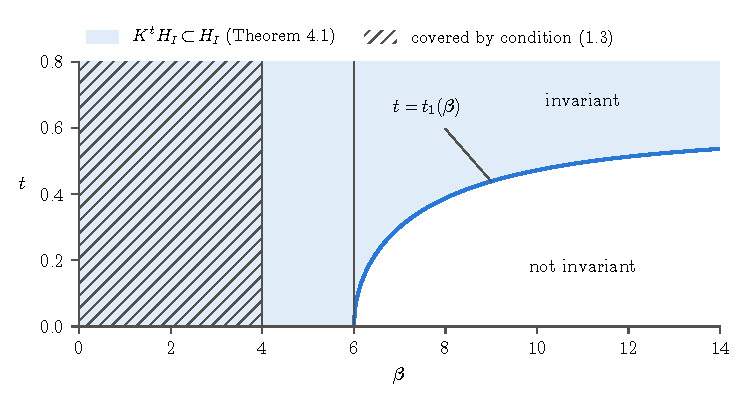
\includegraphics[width=\linewidth]{fig_admissible_times.pdf}
\caption{Admissible times for Example~\ref{ex:beta} ($A=A_\beta$, $B=C=I_2$). Shaded: pairs $(\beta,t)$ with
$K^tH_I\subset H_I$, determined by the criterion $D_t\ge0$ of Theorem~\ref{thm:fixed}. Hatched: pairs covered by the
sufficient condition \eqref{eq:23} of \cite{PSWPN}, i.e.\ $\beta\le4$. For $\beta\le6$ invariance holds for all
$t\ge0$ (Theorem~\ref{thm:semigroup}). For $6<\beta\le14$ it fails for $0<t<t_1(\beta)$ and holds for
$t\ge t_1(\beta)$. The curve $t_1(\beta)$ was computed numerically (Example~\ref{ex:beta} and
Appendix~\ref{app:numerics}).}
\label{fig:times}
\end{figure}

\begin{example}[Scalar noise]\label{ex:scalar}
Let $d=2$, $m=1$, $A=\begin{pmatrix}\frac32&-2\\2&-2\end{pmatrix}$, $B=\begin{pmatrix}1\\0\end{pmatrix}$ and $C=I_2$.
Then $\Tr A=-\frac12$ and $\det A=1$, so the eigenvalues $-\frac14\pm\frac{\sqrt{15}}4i$ have negative real parts and
$A$ is Hurwitz. Moreover $\det[B,AB]=\det\begin{pmatrix}1&\frac32\\0&2\end{pmatrix}=2\neq0$, so $(A,B)$ is
controllable. Since $\frac12(A+A^\tp)=\operatorname{diag}(\frac32,-2)$ and $BB^\tp=\operatorname{diag}(1,0)$,
\[
BB^\tp-\tfrac12(A+A^\tp)=\operatorname{diag}\bigl(-\tfrac12,2\bigr)\not\ge0,\qquad
2BB^\tp-\tfrac12(A+A^\tp)=\operatorname{diag}\bigl(\tfrac12,2\bigr)\ge0 .
\]
So \eqref{eq:23} fails and \eqref{eq:23sharp} holds, and $H_I$ is invariant under every $K^t$ although the noise is
one-dimensional.
\end{example}

%======================================================================
\section{Further remarks}\label{sec:remarks}
%======================================================================

\begin{lemma}[Inner products of Gaussian bumps]\label{lem:bumps}
Let $C',C''$ be symmetric positive definite and $y,y'\in\R^d$. Then $k^{C'}_y\in H_{C''}$ if and only if
$G:=2C'^2-C''^2$ is positive definite. In that case
\[
\ip{k^{C'}_y}{k^{C'}_{y'}}_{C''}=\frac{(\det C')^2}{\det C''\,(\det G)^{1/2}}\exp\bigl(-(y-y')^\tp G^{-1}(y-y')\bigr).
\]
\end{lemma}

\begin{proof}
By \eqref{eq:kernelFT}, $|\hatf{k^{C'}_y}|^2w_{C''}=\kappa_{C'}^2\exp(-\frac14\xi^\tp G\xi)$, which is integrable if and
only if $G>0$. If $G>0$, then \eqref{eq:normC} and \eqref{eq:gauss} with $P=\frac14G$ give
\[
\ip{k^{C'}_y}{k^{C'}_{y'}}_{C''}=(2\pi)^{-d}\frac{\kappa_{C'}^2}{\kappa_{C''}}\int e^{-\frac14\xi^\tp G\xi-i\xi\cdot(y-y')}\dd\xi
=(2\pi)^{-d}\frac{\pi^d(\det C')^2}{\pi^{d/2}\det C''}\,\pi^{d/2}2^d(\det G)^{-1/2}e^{-(y-y')^\tp G^{-1}(y-y')},
\]
and $(2\pi)^{-d}\pi^d2^d=1$.
\end{proof}

\begin{remark}[Why kernel expansions cannot detect non-invariance]\label{rem:sections}
By \cite[Proposition~4.1]{PSWPN}, $K^tk^C_z=\tau_t\,k^{C_t}_{e^{-At}z}$. By Lemma~\ref{lem:bumps}, $K^tk^C_z\in H_C$ if
and only if $2C_t^2-C^2>0$. Now $2C_t^2-C^2=e^{-At}(C^2+D_t)e^{-A^\tp t}$ and $D_t\to0$ as $t\downarrow0$. Hence, for all
sufficiently small $t$, $K^t$ maps $\operatorname{span}\{k^C_z:z\in\R^d\}$ into $H_C$ \emph{regardless} of the sign of
$D_t$. Non-invariance is witnessed only by elements of $H_C$ whose Fourier transforms decay as slowly as membership in
$H_C$ permits within a cone of directions (Lemma~\ref{lem:multiplier}). Such functions are not finite kernel
expansions. This explains why the necessary condition
$\operatorname{span}\{k^{C_t}_x:x\in\R^d\}\subset H_C$ noted in \cite[Remark~4.2]{PSWPN} is too weak to decide the
question.
\end{remark}

\begin{remark}[Consistency with {\cite[Proposition~4.1]{PSWPN}}]\label{rem:consistency}
By Corollaries~\ref{cor:remark42} and~\ref{cor:inclusion}, $H_{\Ct}\subset H_{C_t}$ with
$\|g\|_{C_t}^2\le(\det\Ct/\det C_t)\|g\|_{\Ct}^2$. Together with Theorem~\ref{thm:range} this gives
\[
\|K^tf\|_{C_t}^2\le\frac{\det\Ct}{\det C_t}\,\taut\,\|f\|_C^2
=\frac{\det(C^2+4\Sigma(t))^{1/2}}{\det(C^2+2\Sigma(t))^{1/2}}\cdot\frac{\det C}{\det(C^2+4\Sigma(t))^{1/2}}\,\|f\|_C^2
=\tau_t\,\|f\|_C^2 ,
\]
which is exactly the bound of \cite[Proposition~4.1]{PSWPN}. Thus Theorem~\ref{thm:range} refines that proposition,
and the only loss in the argument of \cite{PSWPN} is the inclusion $H_{\Ct}\subsetneq H_{C_t}$. On kernel sections,
Theorem~\ref{thm:range} reads $\ip{K^tk^C_z}{K^tk^C_{z'}}_{\Ct}=\taut\,k^C(z,z')$. This also follows directly from
\cite[Proposition~4.1]{PSWPN} and Lemma~\ref{lem:bumps}, because $2C_t^2-\Ct^{\,2}=e^{-At}C^2e^{-A^\tp t}$.
\end{remark}

\begin{remark}[Deterministic linear flows]\label{rem:composition}
For $B=0$ we have $\Sigma(t)=0$ and $K^tf=f\circ e^{At}$. The proof of Theorem~\ref{thm:fixed} works verbatim with $e^{At}$
replaced by an arbitrary invertible matrix $E$. It shows that the composition operator $f\mapsto f\circ E$ maps $H_C$
into itself if and only if $EC^2E^\tp\le C^2$, i.e.\ $\|C^{-1}EC\|\le1$, and that its norm is then $|\det E|^{-1/2}$.
For the Fock space of entire functions, bounded composition operators were characterized in
\cite{CarswellMacCluerSchuster}; there, too, the symbol must be an affine map whose linear part is a contraction.
\end{remark}

We finally record what the method gives for other translation-invariant kernels. Let $\varphi\colon\R^d\to\R$ be
continuous, integrable and positive definite, with $\hatf\varphi$ continuous, integrable and strictly positive. Let
$H_\varphi$ denote the RKHS of $(x,y)\mapsto\varphi(x-y)$. By \cite[Theorem~10.12]{Wendland},
$H_\varphi=\{f\in C(\R^d)\cap L^2(\R^d)\ \text{real-valued}:\ \int|\hatf f|^2/\hatf\varphi<\infty\}$, with
$\ip fg_{H_\varphi}=(2\pi)^{-d}\int\hatf f\,\overline{\hatf g}/\hatf\varphi$ in our normalization of the Fourier
transform. For $\varphi(z)=\exp(-z^\tp C^{-2}z)$ this is Lemma~\ref{lem:fourier}.

\begin{proposition}\label{prop:general}
Let $\varphi$ be as above and $t\ge0$, and put
\[
m_t(\eta):=\frac{\hatf\varphi(\eta)\,\exp\bigl(-\eta^\tp\Sigma(t)\eta\bigr)}{\hatf\varphi\bigl(e^{A^\tp t}\eta\bigr)},\qquad\eta\in\R^d .
\]
Then $K^tH_\varphi\subset H_\varphi$ if and only if $\sup_\eta m_t(\eta)<\infty$, and in this case
$\|K^t\|_{H_\varphi\to H_\varphi}^2=e^{-t\Tr A}\sup_\eta m_t(\eta)$. For $\varphi(z)=\exp(-z^\tp C^{-2}z)$ one has
$m_t(\eta)=\exp(-\frac14\eta^\tp D_t\eta)$, and Theorem~\ref{thm:fixed}(a),(b) is recovered.
\end{proposition}

\begin{proof}
Elements of $H_\varphi$ are bounded, continuous and in $L^2$, so Lemma~\ref{lem:Kt} applies. The computation in the proof
of Proposition~\ref{prop:norm} gives
$\|K^tf\|_{H_\varphi}^2=(2\pi)^{-d}e^{-t\Tr A}\int|\hatf f(\eta)|^2m_t(\eta)/\hatf\varphi(\eta)\dd\eta$, whenever the
right-hand side is finite, and $K^tf\notin H_\varphi$ otherwise. If $M:=\sup m_t<\infty$, then
$\|K^tf\|_{H_\varphi}^2\le e^{-t\Tr A}M\|f\|_{H_\varphi}^2$. For the reverse inequality, let $\delta>0$ and choose
$\eta_0$ with $m_t(\eta_0)>M-\delta$. The function $m_t$ is continuous and even, so for small $r>0$ the function
$f_r:=(\mathbf 1_{\{|\eta-\eta_0|<r\}\cup\{|\eta+\eta_0|<r\}})^\vee\in H_\varphi\setminus\{0\}$ satisfies
$\|K^tf_r\|^2\ge e^{-t\Tr A}(M-\delta)\|f_r\|^2$.

Suppose now that $\sup m_t=\infty$. For $k\in\mathbb N$ the set $\{m_t>16^k\}$ is open, nonempty and symmetric. Choose a
bounded symmetric set $E_k$ of positive measure inside it, put $a_k:=(\int_{E_k}\hatf\varphi^{-1})^{-1/2}$ and
$F:=\sum_k2^{-k}a_k\mathbf 1_{E_k}$. By Minkowski's inequality, $(\int F^2/\hatf\varphi)^{1/2}\le\sum_k2^{-k}=1$.
Since $\hatf\varphi\in L^1$, the Cauchy--Schwarz inequality gives $F\in L^1$. Also $F\in L^2$, because $\hatf\varphi$ is
bounded by $\|\varphi\|_{L^1}$. As $F$ is real and even, $f:=F^\vee$ belongs to $H_\varphi$. Since $F\ge2^{-k}a_k\mathbf 1_{E_k}$ for every
$k$,
$\int F^2m_t/\hatf\varphi\ge4^{-k}a_k^2\,16^k\int_{E_k}\hatf\varphi^{-1}=4^k$. Hence $K^tf\notin H_\varphi$. The
Gaussian case follows from \eqref{eq:kernelFT} and a direct computation.
\end{proof}

\begin{example}[Sobolev spaces]\label{ex:sobolev}
For $s>d/2$ let $\hatf\varphi(\xi)=(1+|\xi|^2)^{-s}$. This is the Mat\'ern kernel, and $H_\varphi$ is the space of
real-valued functions in the Sobolev space $H^s(\R^d)$, with the norm
$\bigl((2\pi)^{-d}\int|\hatf f|^2(1+|\xi|^2)^s\bigr)^{1/2}$. Since
$\bigl(1+|e^{A^\tp t}\eta|^2\bigr)/\bigl(1+|\eta|^2\bigr)\le\max\{1,\|e^{At}\|^2\}$ and
$\exp(-\eta^\tp\Sigma(t)\eta)\le1$, we get $\sup m_t\le\max\{1,\|e^{At}\|^2\}^s<\infty$. By
Proposition~\ref{prop:general}, $H^s(\R^d)$ is invariant under every $K^t$, for \emph{all} $A$ and $B$, and
$\|K^t\|\le e^{-t\Tr A/2}\max\{1,\|e^{At}\|\}^{s}$. The restriction \eqref{eq:23sharp} is therefore a feature of
Gaussian kernels: their spectral density is itself Gaussian, so the comparison of $\hatf\varphi$ with its dilation
$\hatf\varphi\circ e^{A^\tp t}$ in $m_t$ is governed by a quadratic form.
\end{example}

\begin{remark}[Outlook]
The proofs use that, for \eqref{eq:sde}, $K^t$ acts on Fourier transforms by composition with a linear map followed by
multiplication with a Gaussian.
For state-dependent diffusion coefficients or nonlinear drifts this structure is lost, and we do not know an
analogous characterization of Koopman-invariant Gaussian RKHSs in that generality.
\end{remark}

\appendix

%======================================================================
\section{Numerical checks}\label{app:numerics}
%======================================================================

The identities above were also checked in floating-point arithmetic with two Python scripts (NumPy/SciPy,
fixed random seed), which are provided as supplementary material. No proof in this paper depends on these
checks. The covariance $\Sigma(t)$ was computed with Van Loan's block-exponential formula \cite{VanLoan} on steps of
length at most $0.25$, combined with the recursion $\Sigma(s+h)=\Sigma(h)+e^{Ah}\Sigma(s)e^{A^\tp h}$. The one-step
formula cancels catastrophically for large $t$.
\begin{enumerate}
\item $\Sigma(t)$ agrees with adaptive quadrature to a relative error of at most $2.7\times10^{-13}$ (random
$A\in\R^{3\times3}$, $B\in\R^{3\times2}$, $t\in\{0.3,1.7,4\}$).
\item Identity \eqref{eq:Dint} holds to a relative error of at most $5.2\times10^{-13}$ for three random triples $(A,B,C)$
with $A$ \emph{not} Hurwitz (spectral abscissae $1.645$, $1.556$, $2.043$) and $t\in\{0.05,0.8,2.5\}$. Moreover
$\|t^{-1}D_t-\Lambda_C\|/\max\{1,\|\Lambda_C\|\}\le3.7\times10^{-6}$ at $t=10^{-6}$, consistent with the $O(t)$ remainder.
\item Theorem~\ref{thm:D}(a),(b) for a random Hurwitz $A\in\R^{3\times3}$ and $B\in\R^{3\times1}$: the entries of
$D_t-(P_C-e^{At}P_Ce^{A^\tp t})$ are at most $2.4\times10^{-14}$ in modulus for $t\in\{0.1,1,6\}$, and those of
$AP_C+P_CA^\tp+\Lambda_C$ at most $1.8\times10^{-14}$.
\item Theorem~\ref{thm:range} on kernel sections (random $2\times2$ data, $t\in\{0.2,0.9\}$): the Gram matrix
$\bigl(\ip{K^tk^C_{z_i}}{K^tk^C_{z_j}}_{\Ct}\bigr)_{i,j\le4}$, computed from \cite[Proposition~4.1]{PSWPN} and
Lemma~\ref{lem:bumps}, agrees with $\taut\,(k^C(z_i,z_j))_{i,j}$ to within $3.8\times10^{-14}$. The value
$\|K^tk^C_z\|_C^2=e^{-t\Tr A}\det C\,\det(2C^2+4\Sigma(t)-e^{At}C^2e^{A^\tp t})^{-1/2}$, obtained from
\eqref{eq:normid}, agrees with the value implied by \cite[Proposition~4.1]{PSWPN} to a relative error of
$1.1\times10^{-13}$.
\item Monte Carlo check of \cite[Proposition~4.1]{PSWPN} for Example~\ref{ex:beta} with $\beta=5$ and $t=0.4$, using
$2\times10^6$ exact Gaussian samples of $Z_t$: $0.436373\pm2.2\times10^{-4}$ against the closed form $0.436051$, a
deviation of $1.45$ standard errors.
\item Example~\ref{ex:beta} for $\beta\in\{4,5,6,7,8\}$: \eqref{eq:23} holds only for $\beta=4$, and
\eqref{eq:23sharp} exactly for $\beta\le6$. On $4200$ grid points in $(0,12]$, $D_t$ has no negative eigenvalue for
$\beta\le6$. For $\beta=7$ and $\beta=8$ the grid points with indefinite $D_t$ form an initial segment ending at $0.298$
and $0.385$, respectively. For $\beta\in\{5,6\}$ the matrix $C_t^2-C^2$ of \cite{PSWPN} has a negative eigenvalue
($-1.2\times10^{-2}$, resp.\ $-2.4\times10^{-2}$) at some $t\le0.0124$, although $D_t\ge0$ there. The closed form of $D_t$
in Example~\ref{ex:beta} matches the numerically computed $D_t$ to within $2.5\times10^{-14}$.
\item Figure~\ref{fig:times}: for $320$ values of $\beta\in(6,14]$ the set $\{t\in(0,40]:D_t\ge0\}$, sampled on
$2\times10^5$ grid points, is an interval $[t_1(\beta),40]$; $t_1$ was located by bisection on $\det D_t$ and increases
from $0.053$ at $\beta=6.025$ to $0.537$ at $\beta=14$. For $t\ge40$ the condition of Theorem~\ref{thm:D}(c) holds.
\item Example~\ref{ex:scalar}: eigenvalues $-0.25\pm0.968i$, $\operatorname{rank}[B,AB]=2$,
$\lambda_{\max}(\frac12(A+A^\tp)-BB^\tp)=0.5$, $\lambda_{\max}(\frac12(A+A^\tp)-2BB^\tp)=-0.5$, and
$\lambda_{\min}(D_t)\ge0$ on $3000$ grid points in $(0,10]$.
\item Proposition~\ref{prop:general}, Gaussian case: for random $A\in\R^{3\times3}$, $B\in\R^{3\times2}$ and $C$,
$t\in\{0.3,1.2\}$, and $1000$ random $\eta$, the quantities $\log m_t(\eta)$ and $-\frac14\eta^\tp D_t\eta$ agree to a
relative error of $3.2\times10^{-14}$.
\item Example~\ref{ex:sobolev}: for a random $A\in\R^{2\times2}$ that is not Hurwitz (spectral abscissa $0.857$),
$B\in\R^{2\times1}$, $s=1.3$ and $t\in\{0.5,2\}$, the bound $m_t(\eta)\le\max\{1,\|e^{At}\|^2\}^s$ holds at
$8.04\times10^4$ points $\eta$ with $10^{-3}\le|\eta|\le10^{6}$.
\end{enumerate}
In total the script for items 1--6 and 8--10 performs $38$ automated checks, all of which pass.

\subsection*{Data availability}
No data were generated or analyzed. The scripts used for Appendix~\ref{app:numerics} and Figure~\ref{fig:times} are
provided as supplementary material.

\begin{thebibliography}{99}

\bibitem{Aronszajn}
N.~Aronszajn, \emph{Theory of reproducing kernels}, Trans.\ Amer.\ Math.\ Soc.\ \textbf{68} (1950), 337--404.

\bibitem{CarswellMacCluerSchuster}
B.~J.~Carswell, B.~D.~MacCluer, and A.~Schuster, \emph{Composition operators on the Fock space}, Acta Sci.\ Math.\
(Szeged) \textbf{69} (2003), 871--887.

\bibitem{Klus}
S.~Klus, I.~Schuster, and K.~Muandet, \emph{Eigendecompositions of transfer operators in reproducing kernel Hilbert
spaces}, J.\ Nonlinear Sci.\ \textbf{30} (2020), 283--315.

\bibitem{Koehne}
F.~K\"ohne, F.~Philipp, M.~Schaller, A.~Schiela, and K.~Worthmann, \emph{$L^\infty$-error bounds for approximations of
the Koopman operator by kernel extended dynamic mode decomposition}, preprint, arXiv:2403.18809 (2024).

\bibitem{Koopman}
B.~O.~Koopman, \emph{Hamiltonian systems and transformation in Hilbert space}, Proc.\ Natl.\ Acad.\ Sci.\ USA
\textbf{17} (1931), 315--318.

\bibitem{Kostic}
V.~Kostic, P.~Novelli, A.~Maurer, C.~Ciliberto, L.~Rosasco, and M.~Pontil, \emph{Learning dynamical systems via Koopman
operator regression in reproducing kernel Hilbert spaces}, Advances in Neural Information Processing Systems
\textbf{35} (2022), 4017--4031.

\bibitem{Mauroy}
A.~Mauroy, I.~Mezi\'c, and Y.~Susuki (eds.), \emph{The Koopman Operator in Systems and Control}, Lecture Notes in
Control and Information Sciences, Springer, Cham, 2020.

\bibitem{PaulsenRaghupathi}
V.~I.~Paulsen and M.~Raghupathi, \emph{An Introduction to the Theory of Reproducing Kernel Hilbert Spaces}, Cambridge
Studies in Advanced Mathematics, vol.~152, Cambridge University Press, Cambridge, 2016.

\bibitem{PhilippACHA}
F.~Philipp, M.~Schaller, K.~Worthmann, S.~Peitz, and F.~N\"uske, \emph{Error bounds for kernel-based approximations of
the Koopman operator}, Appl.\ Comput.\ Harmon.\ Anal.\ \textbf{71} (2024), 101657.

\bibitem{PSWPN}
F.~Philipp, M.~Schaller, K.~Worthmann, S.~Peitz, and F.~N\"uske, \emph{Invariance of Gaussian RKHSs under Koopman
operators of stochastic differential equations with constant matrix coefficients}, Proc.\ Appl.\ Math.\ Mech.\
(PAMM) \textbf{25} (2025), no.~1, e202400127; arXiv:2405.14429.

\bibitem{SHS}
I.~Steinwart, D.~Hush, and C.~Scovel, \emph{An explicit description of the reproducing kernel Hilbert spaces of
Gaussian RBF kernels}, IEEE Trans.\ Inform.\ Theory \textbf{52} (2006), 4635--4643.

\bibitem{VanLoan}
C.~F.~Van~Loan, \emph{Computing integrals involving the matrix exponential}, IEEE Trans.\ Automat.\ Control
\textbf{23} (1978), 395--404.

\bibitem{Vatiwutipong}
P.~Vatiwutipong and N.~Phewchean, \emph{Alternative way to derive the distribution of the multivariate
Ornstein--Uhlenbeck process}, Adv.\ Difference Equ.\ (2019), Paper No.~276.

\bibitem{Wendland}
H.~Wendland, \emph{Scattered Data Approximation}, Cambridge Monographs on Applied and Computational Mathematics,
vol.~17, Cambridge University Press, Cambridge, 2005.

\bibitem{WilliamsEDMD}
M.~O.~Williams, I.~G.~Kevrekidis, and C.~W.~Rowley, \emph{A data-driven approximation of the Koopman operator:
extending dynamic mode decomposition}, J.\ Nonlinear Sci.\ \textbf{25} (2015), 1307--1346.

\bibitem{WilliamsKernel}
M.~O.~Williams, C.~W.~Rowley, and I.~G.~Kevrekidis, \emph{A kernel-based method for data-driven Koopman spectral
analysis}, J.\ Comput.\ Dyn.\ \textbf{2} (2015), 247--265.

\end{thebibliography}

\end{document}
